\chapter{Potentiometer Linearity}\label{potentiometerLin} 
\textbf{Name: Group 630}\\
\textbf{Date: 15/03 - 2016}

\subsubsection{Purpose}
Finding the linearity accuracy of the potentiometer.

\subsubsection{Setup}
\begin{figure}[H]
  \centering
	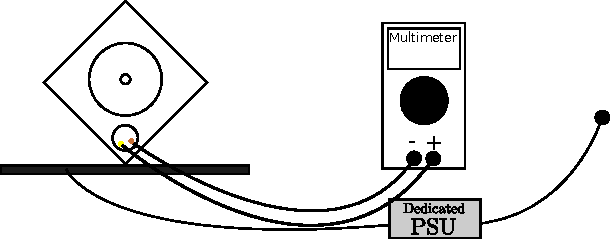
\includegraphics[scale=1]{figures/LabSetupLinearityTest.pdf}
	\caption{Setup diagram}
	\label{LabSetupRangeTest}
\end{figure}\vspace{-5mm}

\subsubsection{List of Equipment}
\begin{table}[H]
	\begin{tabular}{|l|l|p{4.3cm}|}
		\hline%------------------------------------------------------------------------------------------------------------
		\textbf{Instrument}                                  &  \textbf{AAU-no.}  &  \textbf{Type}                       \\
		\hline%------------------------------------------------------------------------------------------------------------
		Multimeter                                           &  TBD           &  Fluke		                   \\
		\hline%------------------------------------------------------------------------------------------------------------
		Dedicated Power Supply of Cubli \small{(24 V - 3 A)} &                    &  XP Power, AEB70US24                 \\
		\hline%------------------------------------------------------------------------------------------------------------
		Digital Protractor                                   &  None               &  TBD\fxnote{find the probe used}     \\
		\hline%------------------------------------------------------------------------------------------------------------
	\end{tabular}
\end{table}

\subsubsection{Procedure}
\begin{enumerate}
  \item Make the setup with connections as seen on \figref{LabSetupRangeTest}, with minus on brown and plus on yellow of the potentiometer.
  \item Setting the multimeter to measure DC mV.
  \item Balance the frame in upright equilibrium position measuring the angle and voltage.
  \item Measuring every 10 degree the voltage of the potentiometer around Equilibrium point and also min and max angle voltage.
\end{enumerate}


\subsubsection{Results}
\begin{table}[H]
	\begin{tabular}{|l|l|p{4.3cm}|}
		\hline%------------------------------------------------------------------------------------------------------------
		\textbf{Angle form equilibrium degrees}       &  \textbf{mV}         \\
		\hline%------------------------------------------------------------------------------------------------------------
		-41,7                                         & 0,066               \\
		\hline%------------------------------------------------------------------------------------------------------------
		-40,0 										  & 0,067               \\
		\hline%------------------------------------------------------------------------------------------------------------
		-38,5                              			  & 4,25               \\
		\hline%------------------------------------------------------------------------------------------------------------
		-30,0                              			  & 50,55               \\
		\hline%------------------------------------------------------------------------------------------------------------
		-20,0                                         & 103,66               \\
		\hline%------------------------------------------------------------------------------------------------------------
		-10,0 										  & 159,20               \\
		\hline%------------------------------------------------------------------------------------------------------------
		0                               			  & 213,64               \\
		\hline%------------------------------------------------------------------------------------------------------------
		10,0                                          & 264,66               \\
		\hline%------------------------------------------------------------------------------------------------------------
		20,0 										  & 317,95               \\
		\hline%------------------------------------------------------------------------------------------------------------
		30,0                              			  & 370,74               \\
		\hline%------------------------------------------------------------------------------------------------------------
		40,0                                          & 425,10               \\
		\hline%------------------------------------------------------------------------------------------------------------
		48,65 										  & 472,11               \\
		\hline%------------------------------------------------------------------------------------------------------------		
	\end{tabular}
\end{table}
	
			
\subsubsection{Results in a graf}
\begin{figure}[H] 
	\centering 
	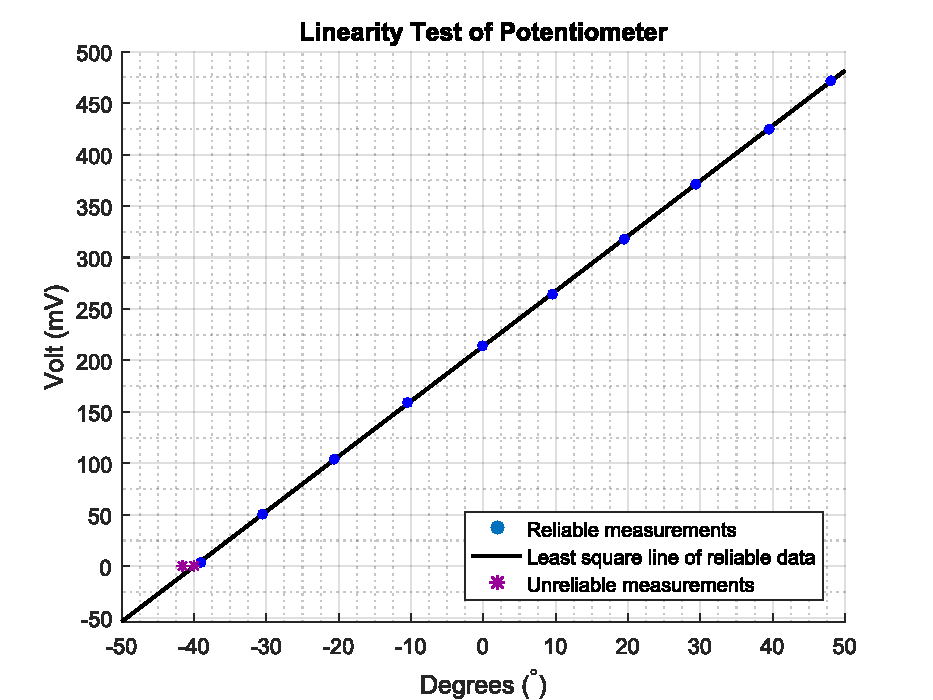
\includegraphics[scale=0.7]{figures/linearityOfPotmeterTest2-1}
	\caption{Raw test data plot}
	\label{linearityOfPotmeterTest2-1}
\end{figure}

\subsubsection{Results}
\begin{table}[H]
	\begin{tabular}{|l|l|p{4.3cm}|}
		\hline%------------------------------------------------------------------------------------------------------------
		\textbf{Equilibrium range degrees}       &  \textbf{mV}         \\
		\hline%------------------------------------------------------------------------------------------------------------
		-0,44                               			  & 211,80               \\
		\hline%------------------------------------------------------------------------------------------------------------
		-0,05                                          & 213,64               \\
		\hline%------------------------------------------------------------------------------------------------------------
		0,053 										  & 217,00              \\
		\hline%------------------------------------------------------------------------------------------------------------
	\end{tabular}
\end{table}

\subsubsection{Results2}
\begin{figure}[H] 
	\centering 
	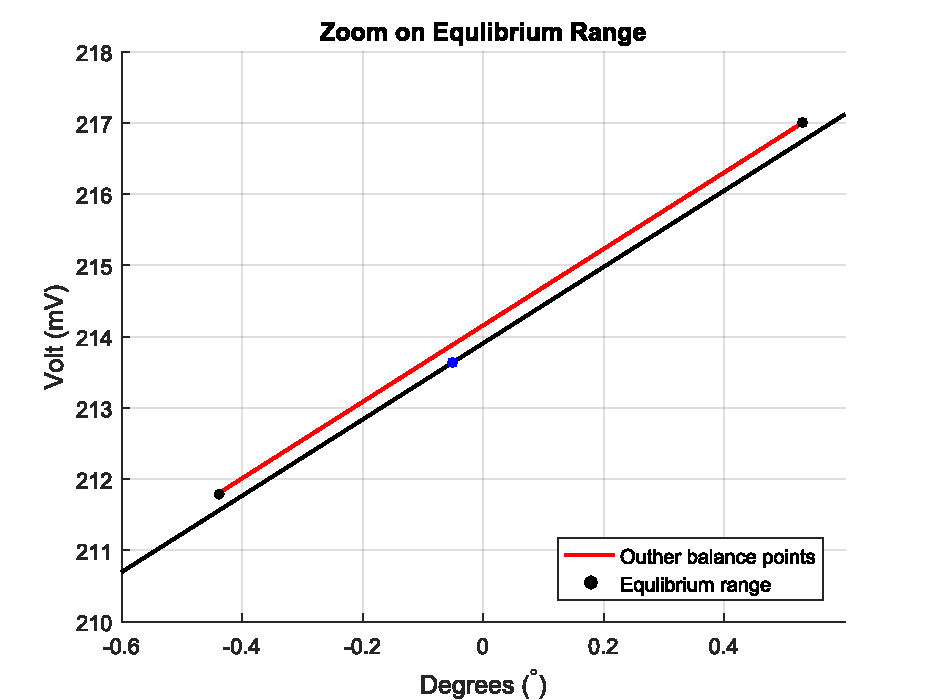
\includegraphics[scale=0.7]{figures/linearityOfPotmeterTest2-2}
	\caption{Raw test data plot}
	\label{linearityOfPotmeterTest2-2}
\end{figure}